\documentclass[border=4pt]{standalone}
\usepackage{tikz}
\usetikzlibrary{arrows,positioning}
\begin{document}
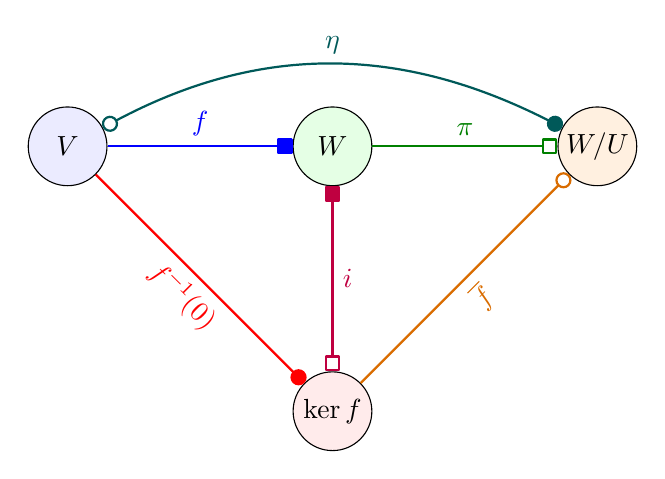
\begin{tikzpicture}[
  node distance=2.35cm,
  object/.style={draw,circle,minimum size=10mm,inner sep=1pt}
]
  \node[object,fill=blue!8] (v) {$V$};
  \node[object,fill=green!10,right=of v] (w) {$W$};
  \node[object,fill=orange!12,right=of w] (q) {$W/U$};
  \node[object,fill=red!8,below=of w] (k) {$\ker f$};

  \draw[blue,line width=.8pt,-square] (v) -- node[above]{$f$} (w);
  \draw[green!50!black,line width=.8pt,-{open square}] (w) -- node[above]{$\pi$} (q);
  \draw[red,line width=.8pt,-*] (v) -- node[below,sloped]{$f^{-1}(0)$} (k);
  \draw[orange!85!black,line width=.8pt,-o] (k) -- node[below,sloped]{$\overline f$} (q);
  \draw[purple,line width=.8pt,{open square}-{square}] (k) -- node[right]{$i$} (w);
  \draw[teal!70!black,line width=.8pt,{o}-{*}] (v) to[bend left=28] node[above]{$\eta$} (q);
\end{tikzpicture}
\end{document}
